\documentclass{article}
\usepackage[utf8]{inputenc}     % for éô
\usepackage[spanish]{babel}     % for proper word breaking at line ends
\usepackage[a4paper, left=1.5in, right=1.5in, top=1.5in, bottom=1.5in]{geometry}
                                % for page size and margin settings
\usepackage{graphicx}           % for ?
\usepackage{amsmath,amssymb}    % for better equations
\usepackage{amsthm}             % for better theorem styles
\usepackage{mathtools}          % for greek math symbol formatting
\usepackage{enumitem}           % for control of 'enumerate' numbering
\usepackage{listings}           % for control of 'itemize' spacing
\usepackage{todonotes}          % for clear TODO notes
\usepackage{hyperref}           % page numbers and '\ref's become clickable
\usepackage{natbib}
\usepackage{subfig}				 % many images in just one figure
\usepackage{indentfirst}		 % package to make first paragraph always indented
\usepackage{float}				 % force figure position(lets use [H])
%%%%%%%%%%%%%%%%%%%%%%%%%%%%%%%%
%% SET TITLE PAGE VALUES HERE %%
%%%%%%%%%%%%%%%%%%%%%%%%%%%%%%%%
%             ||               %
%             ||               %
%             \/               %

\def\thesistitle{Crecimiento y caracterización de láminas delgadas con memoria de
forma de alta temperatura Ni-Ti-Zr mediante sputtering.}
\def\thesissubtitle{Algún día aquí habrá un abstract.}
\def\thesisauthorfirst{Fernando Andres Del Fedele}
\def\thesisauthorsecond{Duck}
\def\thesissupervisorfirst{Dr. Lucio Manuel Isola}
\def\thesissupervisorsecond{Lic. Bruno Federico Malvasio}
\def\thesissecondreaderfirst{prof. dr. Louie}
\def\thesisdate{February 2049}


%             /\               %
%             ||               %
%             ||               %
%%%%%%%%%%%%%%%%%%%%%%%%%%%%%%%%
%% SET TITLE PAGE VALUES HERE %%
%%%%%%%%%%%%%%%%%%%%%%%%%%%%%%%%


%% FOR PDF METADATA
\title{\thesistitle}
\author{\thesisauthorfirst\space\thesisauthorsecond}
\date{\thesisdate}

%% TODO PACKAGE
\newcommand{\towrite}[1]{\todo[inline,color=yellow!10]{TO WRITE: #1}}

%% THEOREM STYLES
\newtheorem{theorem}{Theorem}[section]
\newtheorem{corollary}{Corollary}[theorem]
\newtheorem{lemma}[theorem]{Lemma}
\newtheorem{proposition}[theorem]{Proposition}

\theoremstyle{definition}
\newtheorem{definition}[theorem]{Definition}

\theoremstyle{remark}
\newtheorem*{remark}{Remark}


%% MATH OPERATORS
\DeclareMathOperator{\supersine}{supersin}
\DeclareMathOperator{\supercosine}{supercos}

%%%%%%%%%%%%%%%%%%%%%%%

\begin{document}
\begin{titlepage}
	\thispagestyle{empty}
	\newcommand{\HRule}{\rule{\linewidth}{0.5mm}}
	\center
	\textsc{\Large Universidad Nacional de Rosario}\\[.7cm]
	
\includegraphics[width=25mm]{img/fceia.jpg}\\[.5cm]
	\textsc{Facultad de Ciencias Exactas, Ingeniería y Agrimensura}\\[0.5cm]
	
	\HRule \\[0.4cm]
	{ \huge \bfseries \thesistitle}\\[0.1cm]
	\textsc{\thesissubtitle}\\
	\HRule \\[.5cm]
	\textsc{\large Tesis para la Licenciatura en Física}\\[.5cm]
	
	\begin{minipage}{0.4\textwidth}
	\begin{flushleft} \large
	\emph{Autor:}\\
	\thesisauthorfirst\space
	\end{flushleft}
	\end{minipage}
	~
	\begin{minipage}{0.4\textwidth}
	\begin{flushright} \large
	\emph{Director:} \\
	\thesissupervisorfirst\space
	\emph{Codirector:} \\
	\thesissupervisorsecond\space
	\end{flushright}
	\end{minipage}\\[4cm]
	\vfill
	{\large \thesisdate}\\
	\clearpage
\end{titlepage}

\tableofcontents

\newpage
\section{Introducción}
\towrite{set all margins, font and line interspacing}

\subsection{Motivación}

\subsubsection{Materiales con memoria de forma}

Los materiales con memoria de forma, de aquí en adelante \textit{SMA} (del inglés, Shape Memory Alloys) son aleaciones que pueden recuperar su forma original al ser calentadas luego de haber sufrido una deformación aparentemente plástica. Adicionalmente, estos materiales poseen propiedades interesantes, tales como superelasticidad, alta capacidad de amortiguamiento y alta relación entre la potencia entregada y su peso. Dichas características les permiten permite inducir altas tensiones y deformaciones por transformación.

Se los denomina superelásticos (a veces también denominados pseudo elásticos) ya que pueden retornar a su estado original luego de un estiramiento de hasta 10\% generado por una tensión externa\cite{Rubber}.

Para que un material tenga memoria de forma, debe tener una transformación martensítica, ya que esta es la responsable de las propiedades de superelasticidad y de memoria de forma, como se verá más adelante.

\subsubsection{Aleación NiTi}\label{aleation}
La aleación NiTi en iguales proporciones es un material con memoria de forma. La aleación y sus propiedades fueron descubiertas en 1959. A este compuesto se lo puede hallar bajo el nombre comercial de \textit{Nitinol}, derivado tanto del nombre de la aleación como del lugar donde fue descubierto (Nickel Titanium-Naval Ordnance Laboratory)\cite{Story}. 

Entre sus propiedades pueden destacarse alta tolerancia a altas presiones y deformaciones, alta vida útil antes de sufrir fatiga, biocompatibilidad, alta resistencia a la corrosión química y propiedades eléctricas que acompañan bien a aplicaciones de calentamiento Joule \cite{ThinFilm}.

\subsubsection{Materiales con memoria de forma de alta temperatura}

Las aplicaciones actuales de los SMA están limitadas por debajo de los $100^\circ$ C. Los materiales con memoria de forma de alta temperatura, abreviados como \textit{HTSMA} (del inglés, High Temperature Shape Memory Alloys) son aquellos en los cuales la transformación martensítica sucede a $T > 100^\circ$.

Dentro del grupo de aleaciones con temperaturas de transformación en el rango de $100^\circ$ C y $400^\circ$ C los dos sistemas más estudiados son el resultado de la adición de paladio o platino a la aleación binaria de NiTi. Como alternativa a estos, se presenta la posibilidad de añadir Hf o Zr (ambos agregados en detrimento del Ti)\cite{HTSMA}. En este trabajo en particular se estudiará la adición de Zr ya que tiene un menor costo relativo, y además presenta una alta influencia en las temperaturas de transformación (influencia aún mucho mayor que la generada por el Pd o elPt), lo que permite utilizarlo en concentraciones menores\citep{HTSMA}.

\subsubsection{Aplicaciones}
La aleación de NiTi es presenta usos muy diversos. En hidráulica y neumática es usada en actuadores térmicos y eléctricos. En el ámbito médico, gracias a su biocompatibilidad, se emplea en implantes ortopédicos, ortodoncias y dispositivos intrauterinos, por citar algunas. En estructuras civiles, como puentes por ejemplo, es usado en concreto reforzado inteligente, el cual lo incorpora como cables dentro del concreto. Al detectar una quiebra, los cables se contraen facilitando el arreglo\cite{Engineering}.

Una gran limitación de esta aleación para trabajar como actuador es su baja frecuencia de operación, ya que es difícil transferirle y sacarle calor con suficiente rapidez. Las láminas delgadas permiten sobreponerse a esta dificultad, ya que aumentan la relación de superficie/volumen. Esto permite una mayor disipación del calor, al punto que puede realizarse un ciclo térmico en milisegundos. Esto hace que las peliculas delgadas de este materiales sean adecuadas para fabricar microactuadores\citep{ThinFilm}.

Existe un reciente aumento en el interés, impulsado principalmente por las industrias automotriz y aeroespacial, en desarrollar actuadores de estado sólido basados en aleaciones con memoria de forma que funcionen en rangos de temperaturas superiores.
\subsection{Transformación martensítica}


La transformación martensítica es una transformación de estado sólido, de primer orden, sin difusión atómica y está acompañada por una deformación homogénea de la red que conlleva un cambio en la estructura cristalina \cite{Santamarta}. Dicha transformación ocurre con el desplazamiento coordinado de todos los átomos en distancias del orden de 1 \AA \footnote{Estas transformaciones son llamadas displacivas, ya que los desplazamientos son pequeños en comparación con la distancia interatómica}, manteniendo los átomos su relación con sus vecinos cercanos, es decir que dos átomos que antes de la transformación eran vecinos, seguirán siéndolo luego del cambio de fase\citep{HTSMA} De esta manera, la nueva fase mantiene la misma composición y orden atómico de la fase inicial. La transformación se produce primero preferencialmente en bordes de granos y/o defectos, y luego con un crecimiento de la fase previamente nucleada. Las interfases están constituídas por un plano macroscópicamente invariante, denominado plano de hábito. Esto significa que dos vectores cualesquiera sobre este mantienen sus módulos y orientación relativa constantes durante la transformación \cite{Santamarta}.

Usualmente la fase de mayor temperatura, llamada fase matriz, es cúbica mientras que la fase de menor temperatura, llamada martensita, es monoclínica, teniendo así menor simetría\cite{Malvasio}. Estas transformaciones tienen lugar en un intervalo finito de temperaturas, intervalo en el cual coexisten ambas fases. La transformación directa se induce enfriando el material y la temperatura en la cual comienza el proceso se la denomina $M_s$ (del inglés, martensite start), mientras que la temperatura en la cual termina es llamada $M_f$ (martensite finish). Análogamente, asumamos que el material está completamente en la fase martensítica, esto es $(T < M_f)$. Al calentarlo se produce la transformación inversa en la cual se pasa de martensita a austenita. La temperatura en la cual comienza el proceso es $A_s$(austenite start) y en la cual finaliza es $A_f$(austenite finish).\cite{Santamarta}

Alternativamente, la transformación puede obtenerse aplicando un esfuerzo externo sobre el material, incluso si se está a $T > A_f$, ya que la aplicación de esfuerzo cambia las temperaturas previamente mencionadas. Dicho efecto puede observarse en la Figura \ref{TvsS}. En estos casos una ecuación de Clausius-Clapeyron permite relacionar las variables termodinámicas implicadas en el proceso:
\begin{equation}
	\frac{d\sigma^{A-M}}{dT} = -\frac{\rho \Delta H}{\epsilon T_0}
\end{equation}

Donde $\sigma^{A-M}$ es la tensión para inducir la transformación; $T$ la temperatura; $\rho$ la densidad del material, considerada constante en ambas fases; $\Delta H$ es el cambio de entalpía de la transformación; $T_0$ la temperatura crítica y $\epsilon$ la deformación intrínseca a la transformación \citep{Malvasio}.

\begin{figure}[H]
	\centering
	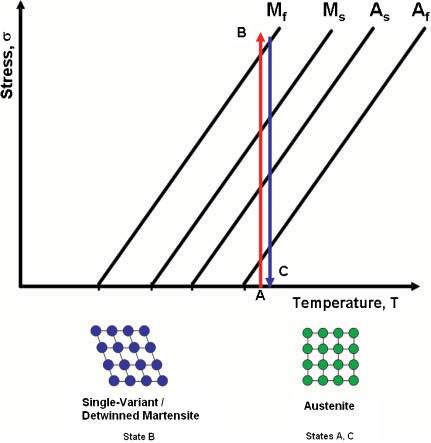
\includegraphics[scale=0.4]{img/StressTransformation.png}
	\caption{Cambio de las temperaturas características con la aplicación de tensión}
	\label{TvsS}
\end{figure}

\subsubsection{Termodinámica de la transformación}
Las transformaciones martensíticas son transformaciones de fase de primer orden sin difusión. Por no tener difusión, no hay cambios de composición y entonces el sistema termodinámico es un sistema monocomponente con dos fases sólidas de diferente estructura.\cite{Santamarta}

Se denomina termoelástica a una transformación martensítica cuando la deformacion que produce la transformación es absorbida en forma elástica por la matriz ($A$, en este caso particular la austenita) que rodea a la martensita (M), de forma que existe un equilibrio termoelástico entre una energía de origen químico y una de origen elástico que controla el avance de la transformación. La fuerza motriz de la transformación es la diferencia de energías libres quiímicas o estructurales de las fases matriz y martensita.
\begin{equation}
	\Delta G^{A \rightarrow M}_q = G^M_q - G^A_q
\end{equation}

Cuando la fase matriz es estable, esto es a altas temperaturas, el delta de energía es positivo. Cuando es estable la fase martensita, a bajas temperaturas el delta es negativo. En un caso ideal, la transformación sucedería a una temperatura $T_0$ en la cual sucedería $\Delta G^{A \rightarrow M}_q = 0$. Sin embargo, la transformación comienza en $M_s < T_0$ y se extiende en un intervalo de temperaturas hasta $M_f < M_s$. Esto se debe a que el sistema necesita una energía suplementaria $\Delta G_q$ para compensar las energías de origen no químico que se oponen a la transformación cuando esta ocurre. Las contribuciones más importantes al término no químico son la deformación eslástica entre la fase matriz y martensita, la cual se alamcena durante la transformación, y un término disipativo que se manifiesta experimentalmente por la presencia de histéresis. El término elástico proveien de la acomodacion de los cambios de forma y volumen asociados a la transformación. El término disipativo incluye energías de fricción en el movimiento de las interfases e interacción de las mismas con otras variantes y/o defectos.

\begin{figure}
	\label{Gibbs}
	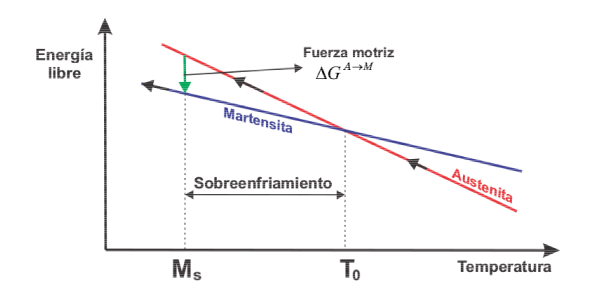
\includegraphics[scale=0.5]{img/Gibbs.png}
	\caption{Energía de la austenita y martensita en función de la temperatura.}
\end{figure}


Mencionadas entonces las fuerzas de origen no químico, la situación de equilibrio para la transformación directa puede expresarse mediante las siguientes ecuaciones, en las cuales los términos están expresados en valor absoluto y los signos se marcan en forma explícita. Para la transformación directa ($A \rightarrow M$):
\begin{equation}\label{GibbsEq1}
	- \Delta G^{A \rightarrow M}_q + \Delta E^{A \rightarrow M}_e + E^{A \rightarrow M}_d = 0 
\end{equation}
Mientras que para la transformación inversa ($M \rightarrow A$)
\begin{equation}
	\Delta G^{M \rightarrow A}_q - \Delta E^{M \rightarrow A}_e + E^{M \rightarrow A}_d = 0 \;\;\;\;\;\;\; T<T_0
\end{equation}
\begin{equation}
	- \Delta G^{M \rightarrow A}_q - \Delta E^{M \rightarrow A}_e + E^{M \rightarrow A}_d = 0 \;\;\;\;\;\;\; T>T_0
\end{equation}

Este conjunto de ecuaciones muestra como cada término influye en las transformaciones directa e inversa. El término elástico se opone a la transformación directa, como indica el signo positivo en \ref{GibbsEq1} y queda almacenado hasta que es recuperado en la inversa, promoviendo de esta manera la retransformación, hecho marcado por el signo negativo en las dos ecuaciones restantes. Si este término es suficientemente grande, la transformación inversa puede comenzar incluso en temperaturas inferiores a $T_0$. El término disipativo siempre se opone al cambio de fase, por este motivo siempre tiene un signo positivo y es el responsable del efecto de histéresis en la transformación.

\todo{Puedo agregar como es la cinética de la transformación en general y Clausus-Clapyeron para tener en cuenta la tensión. ¿Lo hago?}

\subsubsection{Efectos de memoria de forma y superelasticidad como consecuencias de la transformación}

El proceso de memoria de forma comienza a una temperatura $T>A_f$. La forma que tenga el material en este punto es la que será ``recordada''. Luego, se enfría sin esfuerzo hasta una temperatura $T<M_f$. En este enfriamiento se produce la transformación directa de austenita a martensita, formandose la martensita de manera que la energía del sistema se minimice, con lo cual la forma macroscópica del material no cambia.

Siendo la estructura del material la martensita, se aplica un esfuerzo creciente para deformar la aleación. Tanto la deformación elástica de la martensita como la reorientación de las variantes formadas durante el enfriamiento dan lugar a esta deformación. Como estas variantes se mueven con facilidad, se acomodan para concordar con el esfuerzo aplicado. Aún así, si la deformación es muy grande, existe la posibilidad que haya una deformación plástica y el proceso no sea completamente reversible. Una vez relajado el esfuerzo, el material conserva una deformación residual.

Finalmente, al calentarse la aleación a una temperatura $T>A_f$ se da la transformación inversa (martensita a austenita). De esta manera recupera la aleación su forma original, perdiendose la deformación residual. En la figura \ref{3DGraph} puede verse esquematicamente este proceso.

\begin{figure}[H]
	\centering
	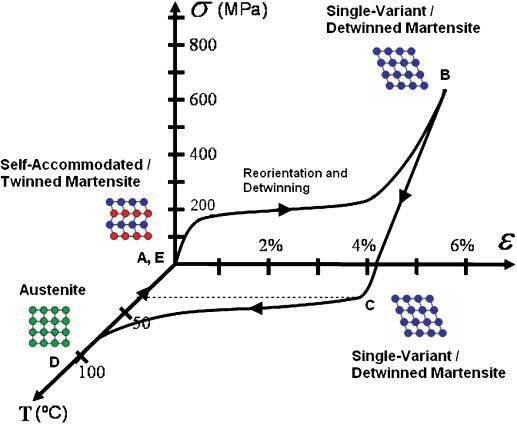
\includegraphics[scale=0.3]{img/3dCycle.png}
	\caption{Diagrama del efecto de memoria de forma en función de tensión y temperatura}
	\label{3DGraph}
\end{figure}


El efecto de superelasticidad cuando se induce la transformación martensítica por tensión, aunque se este a temperatura $T>A_f$. Aplicando tensión al material en austenita, empieza a deformar elásticamente hasta la tensión $\sigma^{p \rightarrow m}$ valor a partir del cual comienza la transformación martensitica.

Al retirarse la tensión, ocurre la transformación inversa, habiendo, al igual que en el caso de memoria de forma, histéresis.

Si la temperatura no es lo suficientemente alta, por ejemplo, $T \approx M_s$, es posible que no todo el material este en estado austenitico y se este en un caso de memoria de forma, con lo cual al relajar la tensión, el material no volvería a su tamaño original.


\subsection{Diagrama de fases del sistema Ni-Ti}
Por debajo de los $650 ^\circ C$ no existe un conocimiento claro del diagrama de equilibrio, aunque se acepta de manera general que la zona de estabilidad de la fase matriz es sumamente estrecha (entre 50.0 y 50.5 \% at. Ni) y que por debajo de $650^\circ$ es una fase metaestable. En la figura \ref{PhaseDiagram} puede verse el diagrama de fases de la aleación. Sólo la fase NiTi es la que presenta una transformación martensítica y, por lo tanto, es la única con el efecto de memoria de forma.

Viendo el diagrama es fácil poder apreciar cuales son las fases que acompañaran al NiTi equiatómico. El $Ti_2Ni$ aparece cuando el contenido de Ti es mayor que el de Ni. Es difícil distinguir del $Ti_4Ni_2O$ debido a que sus parámetros son parecidos. Por otra parte, cuando el contenido de Ni es mayor, la única fase estable es $TiNi_3$.

\begin{figure}[H]
	\centering
	\subfloat[Diagrama completo]{
  		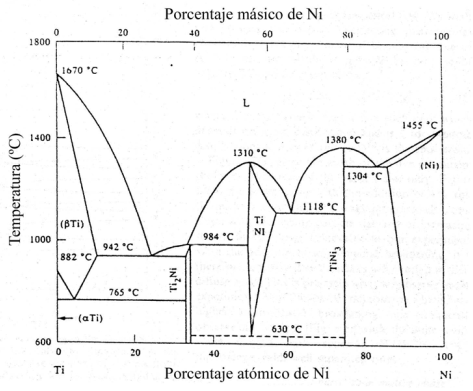
\includegraphics[width=60mm]{img/NiTiPhaseDiagramCompleteSpanish.png}
	}
	\subfloat[Diagrama centrado en NiTi]{
  		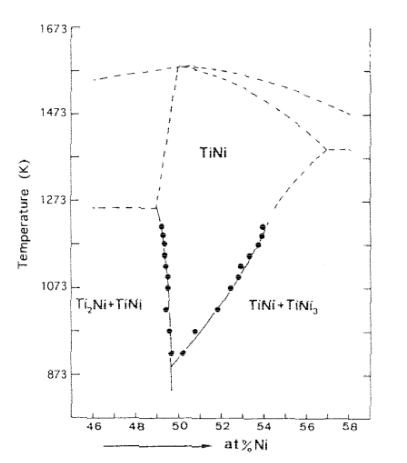
\includegraphics[width=50mm]{img/NiTiphasediagram.png}
	}
	\caption{Diagrama de fases de la aleación Ni-Ti}
	\label{PhaseDiagram}
\end{figure}

La transformación martensítica, como ya se ha mencionado, es una transformación de estado sólido entre dos fases cristalinas. Estas fases han sido objeto de un estudio extensivo desde un punto de vista cristalográfico. En el caso de la aleación binaria NiTi y, en general, las aleaciones de la familia Ni-Ti, se pueden distinguir la fase austenita (B2) y varios tipos de martensita, entre las que podemos destacar la que se conoce como fase R, una fase monoclínica (B19’) y una ortorrómbica (B19). Adicionalmente, se ha reportado una fase adicional H hallada en aleaciones ternarias al agregarse Hf o Zr. A continuación, se realiza una breve descripción de dichas fases.

\subsubsection{Fase B2}
La fase B2 es la correspondiente a la austenita en las aleaciones equiatómicas de NiTi. En la figura \ref{B2phase} puede verse su estructura. Es una estructura cúbica simple ordenada cuyos átomos del motivo están en las posiciones 000 y $\frac{1}{2}\frac{1}{2}\frac{1}{2}$. Esta estructura también es conocida como CsCl.
\begin{figure}[H]
	\centering
	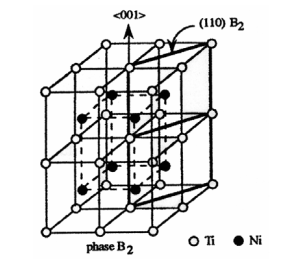
\includegraphics[scale=0.4]{img/B2Phase.png}
	\caption{Estructura de la fase B2}
	\label{B2phase}
\end{figure}

A temperatura ambiente esta fase es metaestable. Se la obtiene desde temperaturas mayores a $650 ^\circ C$ realizando un templado o descenso leve de la temperatura hasta la ambiente.

Los parámetros de red que se pueden encontrar en la literatura pueden variar significativamente, especialmente a causa de los elementos adicionales a la aleación binaria y la cantidad de los mismos. Sin embargo, incluso para la aleación binaria, se pueden hallar valores dispares, generalmente comprendidos entre 2.9 y 3.1 \AA.

\subsubsection{Fase R}
La fase R, es una estructura martensítica correspondiente a una distorsión
ortorrómbica de la malla cúbica (B2) en la dirección $<$111$>$, como se ve en la figura \ref{RPhase}, aunque lo estándar es describirla usando una red hexagonal.
\begin{figure}[H]
	\centering	
	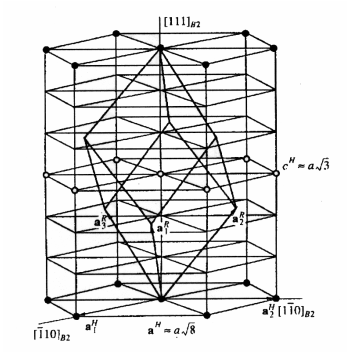
\includegraphics[scale=0.4]{img/RPhase.png}
	\caption{Estructura de la fase R}
	\label{RPhase}
\end{figure}

Esta fase aparece sólo bajo ciertas condiciones antes de la transformación a la fase B19'. Este fenómeno fue interpretado muchas veces como un efecto previo a la transformación, pero actualmente lo aceptado es que es una transformación martensítica de la fase padre B2 a las fase R, que posee una estructura distinta. Los motivos para este análisis son los siguientes
\begin{itemize}
	\item Láminas martensíticas de la fase R son claramente observadas por microscopía electrónica
	\item La transformación directa B2 $\rightarrow$ B19' sólo ocurre en ciertas condiciones
	\item En este proceso también se observan los efectos de memoria de forma y súper elasticidad.
\end{itemize}


Esta fase se ha encontrado en aleaciones ternarias, en las cuales parte del Ni es sustituído por Al, Fe o Co. Se ha hallado que en  aleaciones binarias de NiTi la transformación B2 $\rightarrow$ R $\rightarrow$ B19', que compite con B2 $\rightarrow$ B19', puede favorecerse con ciclado térmico, envejecimiento a $T \approx 400 ^\circ C$ y tratamiento de calor luego de trabajo en frío para generar estructuras dislocadas \citep{Santamarta}\citep{ThinFilm}\cite{TiNi}. 


\subsubsection{Fase B19'}
La fase B19' es una estructura monoclínica. Esta es la fase martensita. En la figura \ref{B19pPhase} se muestra su estructura. Puede haber hasta 24 variantes, según en qué dirección sea la deformación de la fase B2.
\begin{figure}[H]
	\centering
	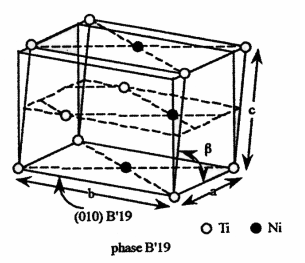
\includegraphics[scale=0.4]{img/B19pPhase.png}
	\caption{Estructura de la fase B19'}
	\label{B19pPhase}
\end{figure}

\subsection{Magnetrón sputtering}
La deposición física por sputtering es una deposición física de vapor usada para generar partículas delgadas. Esta implica emitir material desde el blanco para depositarlo sobre un sustrato. 

 Los átomos o moléculas del material del blanco son arrancados mediante colisiones con los átomos ionizados de un gas inerte, típicamente Argón. Cuando el blanco es el cátodo, se lo denomina \textit{sputtering catódico}. Las partículas abandonan la superficie del target como partículas libres o como una combinación química con las partículas del gas ionizado para luego despositarse sobre una superficie cercana.  Esta "superficie cercana" es justamente un sustrato dedicado a dicha finalidad.
 
Para generar el estado de plasma es necesario alto vacío $\approx 0.5 mTorr$ y un voltaje DC de al menos 500 V.Para aumentar la velocidad de deposición, se aplica un campo magnético alrededor de los blancos. Eso provoca que los electrones orbiten dentro del plasma, ahora concentrado sobre los blancos, y aumenten la cantidad de choques por unidad de tiempo. Es este campo lo que le da el nombre de \textit{Magnetrón sputtering}\citep{Malvasio}\citep{ThinFilm}. En la Figura \ref{sputter} puede verse esquematicamente como es la disposición experimental del proceso.

\begin{figure}[H]
	\centering
	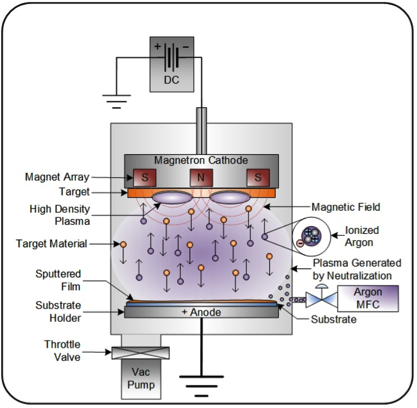
\includegraphics[scale=0.8]{img/diagram-dc-magnatron.png}
	\caption{Esquema del magnetrón sputtering}
	\label{sputter}
\end{figure}

\subsection{Cristalización}

La cristalización es un proceso importante en la fabricación de láminas delgadas de NiTi, ya que es la microestructura la que dicta las propiedades macroscópicas del material y dicha microestructura es fuertemente influenciada por la forma en que se crea el material. A diferencia de la fusión de un material, la cristalización no sucede a una temperatura definida, sino que depende tanto del tiempo como de la temperatura.

La deposición por sputtering debe ser hecha en manera muy cuidadosa, ya que las láminas de NiTi producidas por sputering a temperatura ambiente son sólidos amorfos. Para no obtener fases indeseadas, especialmente si las láminas son ricas en Ni o Ti, estas deben someterse a un tratamiento térmico. En dicho tratamiento deben tenerse en cuenta factores como la energía de activación o la temperatura de cristalización, ya que de lo contrario la lámina puede interactuar con el sustrato sobre el cual está depositada formando una capa interfacial y alterando así sus propiedades.

\subsubsection{Ecuación de Johnshon-Mehl}

 El proceso de cristalización ocurre por nucleación y crecimiento. La nucleación es la formación de la nueva fase. El crecimiento de estos núcleos sucede por la transferencia de átomos a través de la interfase, desde la original hacia las zonas nucleadas. Este proceso continúa hasta que toda la muestra ha cristalizado.En la Figura \ref{cristalization} se muestra esquematicamente este proceso.
 \begin{figure}[H]
 	\centering
	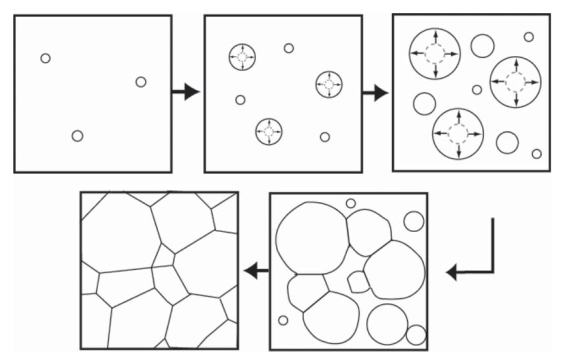
\includegraphics[scale=0.5]{img/cristalization.png}
 	\caption{Esquema del proceso de nucleación y crecimiento.}
	\label{cristalization}
\end{figure} 

Para comenzar el análisis de la transformación, supondremos que la transformación es isotérmica.

Supongamos que la muestra tiene un volumen total $V$, y el volumen transformado de una fase inical $\alpha$ a otra fase $\beta$ es $V_\beta$. Intuitivamente podemos imaginar que el porcentaje de muestra cristalizada en función del tiempo, $X(t) = \frac{V_\beta (t)}{V}$ tendrá un carácter sigmoidal, mostrado esquemáticamente en la Figura \ref{cvst}

 \begin{figure}[H]
 	\centering
	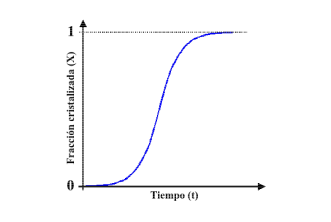
\includegraphics[scale=0.5]{img/cristalization_vs_tiempo.png}
 	\caption{Porcentaje de muestra transformado en función del tiempo}
	\label{cvst}
\end{figure} 

La rapidez con que aparecen nuevas partículas transformadas por unidad de volumen se llama velocidad de nucleación y se denota por $I$. Analogamente, se llama velocidad de crecimiento a la velocidad con que aumenta el radio de los núcleos formados y se denota por $\Gamma$.

Para comprender como cristaliza la muestra en su totalidad, empecemos por
considerar el tamaño de una región individual ya en fase $\beta$, es decir, ya cristalizada. La región se forma en un tiempo de incubación $t=\tau$, y luego crece en forma continua. Si la fase inicial y final tienen la misma composición, como es el caso de la transformación martensítica, experimentalmente se observa que en la mayor parte de los casos que cualquier dimensión de la región transformada es una función lineal del tiempo. \todo{citar the theory of transformations}.

Para facilitar el análisis asumiremos una velocidad de crecimiento isotrópica $\Gamma$, lo que implica que las regiones transforman con simetría esférica. Hay que destacar que no se pierde mucha generalidad con esta aprocimación aunque este no suela ser el caso. Con estás hipótesis, el volumen $v_\tau$ de una región que transformó en un tiempo de incubación es 
\begin{equation}
	v_\tau = \frac{4}{3}\pi \Gamma^3(t-\tau)^3
\end{equation}

El número de nuevas regiones en la fase $\beta$ nucleadas en un intervalo de tiempo entre $\tau$ y $\tau + d\tau$ es $IV_\alpha d\tau$. Entonces, el volumen transformado en un tiempo t, producto de dichas regiones nucleadas es $v_\tau IV_\alpha d\tau$. Al inicio de la transformación, podemos asumir que la velocidad de nucleación $I$ y la de crecimiento $\Gamma$ son constantes y que como $V_\beta << V_\alpha$ entonces $V_\alpha \approx V$, resulta

\begin{equation}
\label{integral}
	V_\beta = \frac{4}{3}\pi V \int_{\tau = 0}^{t} I\Gamma^3(t-\tau)^3d\tau
\end{equation}

Esta función, llamada función de Johsnon-Mehl, da como resultado que la fracción transformada en función del tiempo es:
\begin{equation}
\label{eq1}
	X_e(t) = \frac{V_\beta (t)}{V} = \frac{\pi}{3}\Gamma^3 I t^4
\end{equation}

En esta ecuación la fracción transformada tiende a infinito con el tiempo. El error no es sorprendente ya que en la hipótesis considerada la transformación recién comenzaba, y de hecho, experimentalmente la ecuación \ref{eq1} describe bien la fracción transformada en el $t \approx 0$. El subíndice e es porque este porcentaje suele llamarse fracción cristalizada extendida.

Para describir mejor el proceso, debemos considerar que los núcleos sí interfieron entre ellos al crecer, esto es equivalente a decir que la transformación sólo puede ocurrir en el volumen aún no transofrmado. Al chocar entre sí dos regiones transformadas, puede ocurrir una de tres cosas:
\begin{itemize}
\item Las regiones pueden unirse y formar una única región
\item Pueden tocarse y seguir creciendo como si nunca hubieran interferido
\item Pueden formar una interfase en la que el crecimiento frena, aunque siga en otras partes
\end{itemize}

De todas estas, la última es la que ocurre en una transformación de estado sólido.

Anteriormente se asumió en forma implicita que la nucleación ocurre en forma aleatoria, aunque esto no es verdad, la hipótesis aún puede ser aplicada. Lo que en verdad sucede es que la nucleación ocurre en sitios preferenciales de la muestra. Sin embargo, dividiendo la muestra en pequeños elementos de volumen, cada elemento contiene muchos de estos sitios preferenciales, con lo cual puede asumirse que cada uno de estos elementos tiene la misma probabilidad de nucleación. Cómo esta nucleación es igualmente probable en todas partes, cuanto mayor sea la fracción cristalizada, mayor es la probabilidad que $dX_e$ sea de lo ya transformado. Describiendo entonces la fracción cristalizada real con respecto a la fracción cristalizada anterior queda:
\begin{equation}
 dX = (1 - X)dX_e
\end{equation}
La solución de está ecuación diferencial es:
\begin{equation}
	X(t)=1-e^{-\frac{\pi}{3}V^3 I t^4}
\end{equation}
Esta ecuación mantiene el comportamiento proporcional a $t^4$ para baja tiempos chicos, pero satura en $X = 1$ para tiempos grandes

\subsubsection{Modelo de Avrami}
En general,la velocidad de nucleación $I$ no es constante. Para corregir este hecho, Avrami consideró que la nucleación sólo ocurre en sitios preferenciales de la muestra que se van agotando con el tiempo. Sea $N_0$ los sitios iniciales de nucleación por unidad de volumen en la muestra, luego de un tiempo t tenemos
\begin{equation}
	N(t) = N_0e^{-\nu t}
\end{equation}
Donde $\nu$ es la velocidad con la que un núcleo cristaliza. Luego, la velocidad de nucleación por unidad de volumen es 
\begin{equation}
	I = -\frac{dN}{dt} = N_0\nu e^{-\nu t} = N\nu
\end{equation}
Sustituyendo esta fórmula en la ecuación \ref{integral} e integrando por partes queda
\begin{equation}
	X = 1-exp \left\lbrace 8\pi N_0\frac{\Gamma^3}{\nu^3} \left[ e^{-\nu t} -1+\nu t -\nu^2t^2/2 + \nu^3 t^3/6 \right] \right\rbrace
\end{equation}

Para valores chicos de $\nu t$ se obtiene nuevamente la ecuación de Johnson-Mehl, pero para valores grandes de $\nu t$ resulta:
\begin{equation}
	X = 1 - exp\left\lbrace -\frac{4}{3} \pi N_0 \nu^3 t^3 \right\rbrace
\end{equation}
En general la fracción cristalizada en función del tiempo sigue la ecuación

\begin{equation}
	X = 1 - e^{-(kt)^n}
\end{equation}

Donde $n$ es el exponente de Avrami y $k$ una constante dependiente de la velocidad de nucleación y crecimiento.
	El exponente de Avrami generalmente toma valores entre 1.5 y 4, y en casos de nucleación tridimensional se restringe a valores entre 3 y 4. Esto debería cubrir los casos en los que la velocidad de nucleación $I$ es una función decreciente en el tiempo, hasta el caso límite ($n = 4$) en que es constante. En el caso de láminas delgadas, el crecimiento en el espesor finaliza rapidamente, con lo cual el proceso es esencialmente bidimensional y $n$ toma valores entre 2 y 3, siendo 3 el caso límite de velocidad de nucleación constante. 
	
Como los procesos de nucleación y crecimientos son procesos activados térmicamente, la constante k puede ser descripta como
\begin{equation}
\label{kvalue}
	k=fe^{-\frac{E_c}{RT}}
\end{equation}

donde f es el llamado factor de frecuencia y $E_c$ la energía de activación.
La cristalización puede ser descripta completamente si se conocen los valores de $n$, $E_c$ y f. Estos parámetros normalmente se hayan midiendo la fracción cristalizada en función del tiempo para procesos isótermicos y ajustando la ecuación convenientemente.

La energía de activación de la cristalización puede usarse para describir la estabilidad térmica de una fase, donde mayores números se corresponden con mayores valores de estabilidad.

\subsubsection{Relación de Kissinger}
Para lograr medir la energía de activación en procesos térmicamente activados, Kissinger desarrolló una formulación teórica sencilla para describir los experimentos en los cuales la temperatura aumenta a ritmo constante. Esta formulación se basa en que la probabilidad de que una región transforme es la misma para todas las partes del volumen sin transformar, esto es, es una transformación homogénea. Entonces, el volumen transformado en un intervalo de tiempo es proporcional al volumen que quedaba en la fase original al comienzo de dicho intervalo, esto es $dV_\beta = k V_\alpha dt$. Esto permite expresar la velocidad de transformación en función del porcentaje transformado mediante la siguiente ecuación diferencial:
\begin{equation}
	\dot{X} = k(1-X)
\end{equation}
cuya solución es
\begin{equation}
	X(t) = 1 - e^{-kt}
\end{equation}
Que es en definitiva un caso particular del modelo de Avrami en el cual $n=1$.
Suponiendo que el aumento de temperatura ocurre en forma constante, como es el caso de un proceso de calorimetría diferencial de barrido, se tiene que:
\begin{equation}
	T(t) = T_0+\alpha t
\end{equation}
Donde $T_0$ es la temperatura incial y $\alpha$ la velocidad de calentamiento. El máximo de la velocidad de reacción $\dot{X}$ ocurre en el pico del barrido, y en la temperatura de este pico ($T_p$) se tiene que $\ddot{X} = 0$.

Con estas consideraciones, y recordando el valor de k de la Ecuación \ref{kvalue} se llega a la ecuación:
\begin{equation}
	fe^{-\frac{E_c}{RT}} = \frac{\alpha E_c}{R T_p^2}
\end{equation}

Aplicando logaritmo natural miembro a miembro para simplificar la expresión se obtiene la relación de Kissinger:
\begin{equation}
	ln(\frac{\alpha}{R T_p^2}) = -\frac{E_c}{RT_p} + cte
\end{equation}

Con los diversos valores de $T_p$ obtenidos de barridos a distintas velocidades $\alpha$ puede graficarse $ln(\frac{\alpha}{R T_p^2})$ vs $T_p^{-1}$, y de la pendiente de esta recta puede obtenerse el valor de la energía de activación, $E_c$
\subsubsection{Relación de Augis-Bennet}
Para conservar el model de Avrami en un proceso a temperatura variable, Augis y Bennet propuesieron un modelo alternativo al de Kissinger. Este considera que el proceso es aproximable por una sucesión de pasos isotérmicos.
De la ecuación \ref{kvalue} y de considerar a la temperatura como una función lineal en el tiempo, podemos definir
\begin{equation}
	u = kt = ft exp \left\lbrace -\frac{E_c}{R(T_0 + \alpha t)} \right\rbrace
\end{equation}

Esto permite reescribir el modelo de Avrami como \todo{es eso lo que reescribo acá?}
\begin{equation}
	X = 1-e^{-u^{n}}
\end{equation}
de donde sale que
\begin{equation}
	\dot{X} = \dot{u}nu^{n-1}(1-X)
\end{equation}
Considerando una vez más que el máximo de la velocidad de la reacción coincide con el pico del del barrido, vuelve a suceder que $\ddot{X}(T_p) = 0$. En este modelo se llega a la siguiente expresión
\begin{equation}
	f^n exp \left\lbrace -\frac{n E_c}{RT_p} \right\rbrace = (\frac{\alpha}{T_p - T_0})^n
\end{equation}

Aplicando logaritmo natural a esta expresión se obtiene la relación de Augis Bennet:
\begin{equation}
	ln(\frac{\alpha}{T_p - T_0}) = -\frac{n E_c}{RT_p} + cte
\end{equation}
Donde la forma de hallar el valor de $E_c$ es similar a la de Kissinger, a partir de la pendiente de la gráfica $ln(\frac{\alpha}{T_p - T_0})$

\section{Técnicas experimentales}

\subsection{Difracción por rayos X}
 La difracción por Rayos X es una técnica para determinar la estructura molecular de un material cristalino. Al recibir la muestra un haz incidente de Rayos X, los electrones lo absorben para luego vibrar a dicha frecuencia como un dipolo, emitiendo así radiación de la misma frecuencia a la incidente. En este proceso se producen fenómenos de difracción e interferencia.  Conociendo las intensidades y los ángulos de dichos haces difractados es posible determinar la estructura del material.
 
\begin{figure}[H]
\centering
\subfloat[Reflexión de Bragg en planos atómicos.]{
  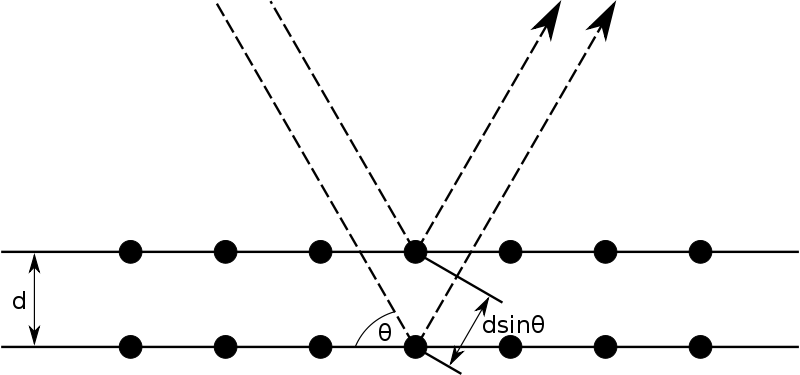
\includegraphics[width=60mm]{img/Bragg.png}
}
\subfloat[Esquema del dispositivo tipo Bragg-Brentano.]{
  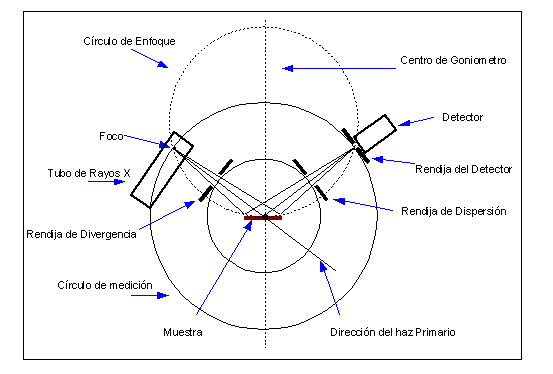
\includegraphics[width=60mm]{img/gonio.png}
}
\end{figure}
 
 Este fenómeno de difracción sucede cuando la longitud de onda de la radiación incidente es comparable a las distancias entre los átomos del material. Está distancia es del orden de 0,15 a 0,4 nm, que en el espectro electromagnético corresponde a los Rayos X, con energías entre 3 y 8 keV. De usarse una longitud mayor de onda, Rayos UV por ejemplo, se obtendría menor resolución y de usarse una menor longitud de onda, se correría el riesgo de alterar la muestra debido a la alta energía que poseería la radiación.
 
 
 Este fenómeno de difracción puede ser explicado mediante la Ley de Bragg. Radiación electromagnética incide en los diferentes planos atómicos, la cual ser re-emitida presentará un fenómeno de difracción e interferencia debido a una diferencia de recorrido. La interferencia será constructiva en caso de que la distancia entre los planos cumpla con
 \begin{equation}
 2d sin \theta =n \lambda; n \in \mathbf{N}
 \end{equation}
 
 
 Luego, la intensidad del haz refractado es medida para diversos ángulos, en este caso $10^{\circ}$ a $120^{\circ}$ y es mostrada en función del parámetro $2\theta$. Al deberse este patrón de intensidades  a factores puramente geométricos de la estructura, se emplea para discernir distintas estructuras y encontrar valores característicos como la distancia entre planos o los parámetros de red de la celda unidad.

 El dispositivo usado para esta medición fue un difractómetro Philips X'Pert Pro X-ray, de tipo Bragg-Brentano en la configuración $\theta - 2\theta$.  Para el análisis de los datos, fue usado el programa \textit{Highscore} con la base de datos \textit{PDF 2004 ICDD}.
 
\subsection{Calorimetría diferencial de barrido}
La calorimetría diferencial de barrido, llamada normalmente DSC (del inglés, differential scanning calorimetry) es una técnica termoanalítica en la cual se mide la diferencia de de calor requerida para calentar una muestra y una referencia como función de la temperatura. La medición suele realizarse en una atmósfera controlada de un gas inerte, y con rampas programas de cambio de temperatura en función del tiempo.  Es necesario destacar que la referencia debe ser inerte en el rango de temperaturas medido.
Esta técnica permite determinar las temperaturas a las cuales ocurren distintos procesos en los materiales, como transformaciones de fase o reacciones químicas. Además, es posible determinar el calor específico y el cambio de entalpía que acompañan las transiciones de primer y segundo orden, ya sean procesos exotérmicos o endotérmicos.

El calorímetro usado fue el model Shimadzu DSC-60, cuyo esquema se muestra en \todo{poner figura}. Para usarlo, se configura un programa que controla la temperatura del bloque calefator ($T_b$), del cual fluye calor a través de una resistencia R hacia la muestra y la referencia, haciendo que la temperatura de la muestra ($T_m$) y la temperatura de la referencia ($T_r$) cambien al igual que $T_b$. La diferencia entre la $T_m$ y $T_r$ es $\Delta T = T_m - T_r$
Cuando la muestra se funde, su temperatura se mantiene constante mientras que la temperatura de la referencia sigue aumentando. Cuando esto sucede, es necesario entregarle mucho más calor a la muestra para que su temperatura se mantenga igual a la de la referencia. En caso de una solidificación, lo inverso ocurre.

El área debajo de los picos registrados es proporcional a la energía calórica necesaria para la transformación o reacción que sucede. En condiciones de presión constante, la energía calórica es igual al cambio de entalpía $\Delta H$ de la muestra.

El equipo trabaja con panes de Al de 3mm de diámetro, dónde se colocan las muestras a ser estudiadas.

\subsection{Deposición por magnetrón sputtering}
Para realizar la deposición se usaron 3 magnetrones modelo \todo{qué modelo?}. Todos están compuestos de la siguiente manera: por el exterior una carcasa de acero inoxidable, que es el ánodo; dentro de ellos se colocan imanes; el blanco, que es a su vez el cátodo, esta sujetado por un acoplamiento magnético al resto de las partes; entre los imanes y el blanco se coloca un anillo de cobre conectado con un sistema de circulación de agua para actuar como refrigerante durante la experiencia. Los blancos usados fueron de titanio, níquel y zirconio.

La deposición fue hecha dentro de una cámara de acero inoxidable, la cual se muestra en la figura \todo{poner figura}. La cámara posee una ventana de cuarzo para poder ver en su interior, sin embargo al avanzar la deposición dicha ventana se contamina y no puede seguir viéndose dentro.

\subsubsection{Atmósfera dentro de la cámara}
La atmósfera dentro de la cámara era de argón a 3mTorr. Se eligió Ar como gas ya que al ser inerte no hay posibilidad que reaccione con alguno de los metales a ser depositados. Para llegar al nivel de vacío requerido, se usó \todo{misma bomba?} una bomba turbomolecular Varian V70 que alcanza un vacío base de $1,5x10^{-10}Torr$. Esta bomba requiere un vacío previo\todo{vacío mínimo?}, para lo cual primeramente se realizó vacío con una bomba mecánica capaz de reducir la presión hasta $10^{-4}Torr$. Para reducir el caudal durante la deposición y así lograr una atmósfera más estable, se colocó una válvula plato entre la bomba turbomolecular y la cámara.

La medición de vacío se realizó con \todo{ver que medidores eran y que medían}
\subsubsection{Sistema eléctrico}
\towrite{Explayarme, eran 3 resistencias y 3 fuentes creo}
\subsubsection{Colocación de las muestras}
Dentro de la cámara se encontraban dos platos metálicos, uno sobre el otro, unidos por un eje. En el inferior se encontraban las muestras y el superior actuaba como pantalla para evitar deposición alguna sobre las muestras hasta que las condiciones sean las adecuadas (presión y potencia estable). Al alcanzarse las condiciones deseadas, se hace girar unicamente el plato superior lo suficiente para que las muestras queden expuestas. Luego giran a velocidad constante de 60rpm en forma conjunta durante la deposición para que esta sea uniforme para todas las muestras.

\subsection{Microscopía electrónica de barrido}
El microscopio electrónico de barrido (SEM, del inglés Scanning Electron Microscope) es un dispositivo que produce imagenes de alta resolución de la superficie de la muestra realizando un escaneo con un haz concentrado de electrones. Dichos electrones interactúan con la muestra produciendo varias señales que contienen información sobre la topografía de la superficie de la muestra y de su composición. Estas posibles señales son electrones secundarios, electrones retrodispersados, rayos X característicos, corriente absorbida y electrones transmitidos, siendo las operatorias más comunes la de electrones secundarios y la de rayos X.

Los electrones secundarios son emitidos por los átomos que ocupan la superficie superior y producen una imagen fácilmente interpretable de la superficie. El contraste de la imagen está determinado por la morfología de la muestra y la resolución de la misma depende del diámetro del haz de electrones primario. Este, en general, es del orden de los nanómetros, controlado por el tipo de generador de los electrones (termoiónicos, vía transistores de efecto de campo (FET)) y la ''óptica” asociada.

La interacción del haz primario con los átomos de la muestra genera transiciones de los electrones entre distintos niveles de energía que dan lugar a la emisión de rayos X que tienen la energía característica del elemento emisor. La detección y medición de la estas energías permite realizar análisis elemental, ya que cada átomo tiene su patrón de emisión característico. Este análisis se denomina espectroscopía EDS.

Como fuente de electrones estos dispositivos tienen distintos tipos de cañones para generar haces de alta o baja energía. En el caso de muestras metálicas, al no haber riesgo de dañar la muestra se usan haces de alta energía para conseguir la mejor resolución posible. Los electrones emitidos pasan a través de una columna en vacío donde el haz inicial es concentrado por lentes electromagnéticas llamadas lentes condensadoras y lente objetivo, con el objetivo de obtener una mejor resolución en la imagen final. Finalmente el haz es direccionado sobre toda la superficie mediante una serie de bobinas deflectoras para generar las interacciones de los electrones con el material y producir las señales antes descriptas. Finalmente, estas señales son captadas por los detectores adosados al equipo

 \begin{figure}[H]
 	\centering
	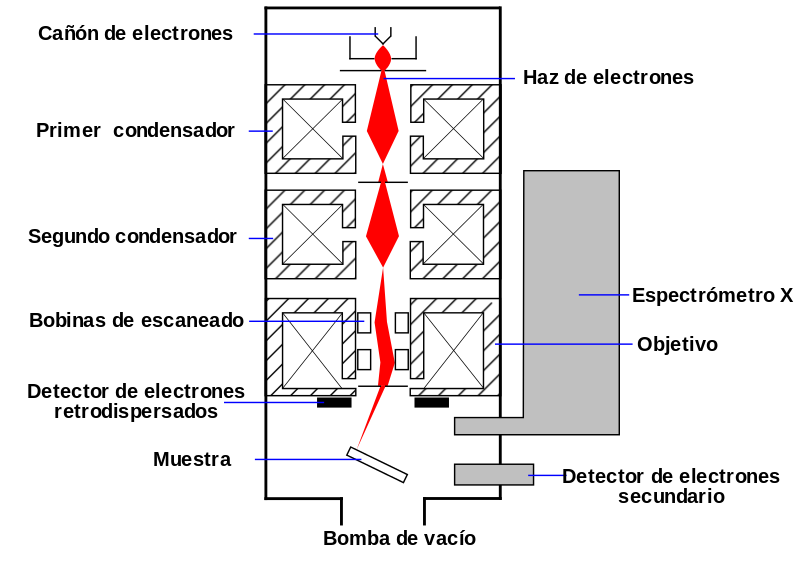
\includegraphics[scale=0.5]{img/SEM.png}
 	\caption{Esquema del tubo de un microscopio electrónico de barrido.}
	\label{SEM}
\end{figure} 

El equipo utilizado es un Leitz Wetzlar AMR1000 con filamento de tungsteno. El detector de rayos X es un modelo Oxforde XMAX. Con dicho detector se realizó un análisis de la composición química de las muestras. Se realizaron dos análisis, uno detectando todos los elementos presentes y otro detectando unicamente Ni, Ti y Zr. Los datos fueron analizados con el software AZtec 3.0.

Para este estudio se armó un portamuestras con \todo{que había acá?}.

Antes de cada medición, se midió la intensidad del pico de rayos X sobre la muestra de Co puro, con el objetivo de estandarizar la corriente del filamento y no medir hasta que esta estuviese estabilizada, asegurando reproducibilidad de los resultados.

\subsection{Resistividad por el método de cuatro puntas}
Al cambiar un material su estructura atómica, lo normal es que muchas de sus propiedades se vean afectadas, entre ellas la resistividad. Si esta transición sucede mientras a través del material circula una corriente eléctrica, puede asociarse un cambio en la resistencia con un cambio de fase. De esta manera, al tener una corriente controlada, al medir la diferencia de potencial es posible determinar donde comienzan y terminan los cambios de fase.

A la lámina delgada se le aplica una corriente alterna constante $I$ a través de dos contactos y con otros dos contactos en la zona de circulación de la muestra se mide la caída de potencial $\delta V$. De estos cuatro contactos deriva el nombre del método. Un esquema de la disposición se muestra en la figura \ref{4puntas}. La lámina es sujetada en una base de cobre, llamada dedo frío, con los cuatro contactos compuestos de un alambre de Constatán soldada a una capa elástica de acero para asegurar un buen contacto eléctrico.

 \begin{figure}[H]
 	\centering
	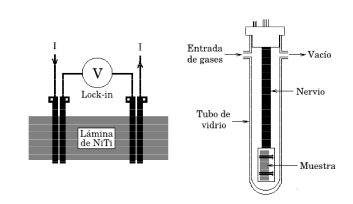
\includegraphics[scale=0.5]{img/r4puntas.png}
 	\caption{Esquema de el sistema empleado para el método de resistividad por  cuatro puntas}
	\label{4puntas}
\end{figure} 

Toda esta estructura se encuentra dentro de un tubo de vidrio cerrado, lo cual permite que el sistema sea sumergido en nitrógeno líquido para trabajar con la muestra a bajas temperaturas. Por arriba, el tubo está cerrado con un tapón de teflón. Este tapón cuenta con un o'ring que garantica el cierre hermético con las paredes del tubo y por cada contacto eléctrico un pequeño o'ring. Los contactos son ajustados por una única tapa superior ajustada por tres tornillos. Los cables que pasan a través del tapón son los siguientes:
\todo{Asegurarme que todas las listas tengan el mismo formato}
\begin{itemize}
\item Dos contactos por los cuales circula la corriente 
\item Dos contactos para medir la diferencia de potencial
\item Dos contactos para conexión del Variac
\item Un contacto para la termocupla
\end{itemize}


Dentro del dedo frío hay una resistencia eléctrica alimentada por transformador Variac, calentando la muestra por efecto Joule. La temperatura se mide con una termocupla sobre el dedo frío. Al estar la muestra cubierta con lana de alumina, esta intercambia calor unicamente con el dedo frío, por lo cual puede considerarse que tanto muestra como dedo frío están siempre a la misma temperatura.

En la parte superior del tubo hay dos aberturas laterales. Una de ellas está conectada a un acople T que conecta un tubo de Ar y otro de He. La otra abertura se conecta con una bomba de vacío.

Todas las mediciones se realizaron en una atmósfera de He a 660 Torr y un vacío base de 20 mTorr. Se trabajó en una atmósfera inerte para evitar que la condensación de la humedad ambiente a bajas temperaturas afectase la medición, y se eligió atmósfera de He en lugar de Ar ya que el último se condensa dentro del rango de temperaturas en el cual se trabajó.

Al ser la muestra un material conductor, la diferencia de potencial medida es muy pequeña (orden de los $\mu V$) el instrumento para llevar a cabo la medición debe ser de alta precisión y con filtros de ruido. El equipo usado para esta tarea fue un amplificador Lock-in modelo Sr-510 Stanford Research. En los contactos exteriores se aplico una corriente una corriente de aproximadamente $10mA$, generada con un generador de señal operando a un 1 $kHz$ a través de una resistencia de 1$k\Omega$. El dispositivo estaba conectado a un sistema de adquisición de datos en una computadora. La temperatura fue medida a través de una termocupla tipo K conectada a una punta fría y a un multímetro Agilent.

\todo{agregar ¿aca? rangos de temperatura y medición ejemplo}

\subsection{Microscopía electrónica de transmisión}
La microscopía electrónica de transmisión, conocida normalmente como \textbf{TEM} (del inglés, \textbf{T}ransmission \textbf{E}lectron \textbf{M}icroscopy) es una técnica de microscopía en la cual un haz de electrones atraviesa una muestra para formar una imagen. El poder de resolución de esta técnica se sitúa en el orden de $1 \AA$, resolución lograda ya que la onda de de Broglie de electrones muy energéticos es considerablemente menor que aquella de la luz visible. Para realizar esta técnica se requiere que la muestra tenga un grosor menor a $100 nm$, debido al escaso poder de penetración de los electrones.

Un microscopio de este tipo consiste de un cañon de electrones y de un cojunto de lentes magnéticas dentro de una columna de vacío. Dicho esquema se muestra en la Figura \ref{TEM}. La disposición de las lentes magnéticas para controlar el haz es similar a la disposición de lentes ópticas en un microscopio común.

 \begin{figure}[H]
 	\centering
	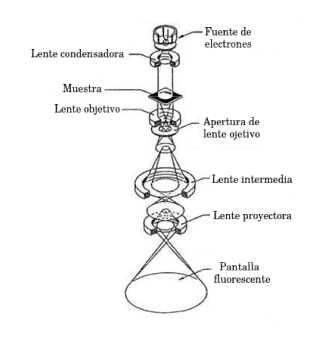
\includegraphics[scale=0.5]{img/TEM.png}
 	\caption{Esquema del tubo de un microscopio electrónico de transmisión.}
	\label{TEM}
\end{figure} 

Una lente magnética es un dispositivo que permite el foco o la deflección de partículas con carga usando la fuerza de Lorentz. Normalmente consisten de bobinas por las cuales circula corriente rodeadas por materiales ferromagnéticos diseñados para concentrar el campo magnético en un espacio confinado. La distancia focal de estas lentes es regulado variando la corriente que circula por las bobinas.

La lente condensadora permite producir un haz de electrones colimado incidente sobre la muestra. Luego de atravesar la muestra, el haz de electrones atraviesa una lente objetivo, cuya tarea es formar una imagen magnificada hasta 40 veces en el plano focal de la siguiente lente, la lente intermedia. Esta lente produce una magnificación aún mayor que llega a la lente proyectora. Esta última lente reproduce la imagen, una vez más aumentada, sobre el receptor final de imagen, normalmente una pantalla fluorescente.

\subsubsection{Preparación de las muestras}

Para que las muestras sean lo suficientemente finas para el TEM, es necesario realizarlas algún tipo de tratamiento. Normalmente se realiza un pulido electrolítico. Esto es, se establece una celda eletrolítica donde la muestra es el ánodo y se aplica un voltaje para disolverla en forma controlada hasta obtener el espesor deseado. En el presente trabajo, al ser las muestras demasiado frágiles se opto por el método de adelgazamiento iónico. \todo{Hay algún mejor nombre?}

Este proceso consiste en acelear iones de un determinado gas, en este caso y normalmente Ar, en un alto vacío en la dirección del sustrato. Este choque de iones va liberando moléculas de la capa superior de la muestra, proceso que se mantiene hasta que se obtiene el espesor deseado. En el caso de muestras cristalinas, se produce la amorfización de las capas cercanas a la superficie (unos pocos nanómetros). Sin embargo, la estructura cristalina original permanece dentro de la muestra y las capas amorfas no interfieren con la observación.


\section{Resultados obtenidos}

\subsection{Deposición de las láminas delgadas}
Se realizaron dos deposiciones para obtener láminas delgadas de NiTiZr. En la tabla \ref{algo} se encuentran los valores de la corriente, voltaje y potencia de cada blanco en ambas deposiciones. Los errores corresponden a las variaciones observadas durante las deposiciones, que era mayor al error de los instrumentos. Al no tener un equipo que estabilice la potencia en función de la tensión de línea, el proceso se hacía manualmente y cada 10 minutos se registraba la potencia de cada magnetrón.

En ambos casos se trabajo con un vacío base de $3 x 10^{-3}mTorr$ y una atmósfera de Ar a $3 mTorr$. Para que la deposición fuese uniforme, el plato de la cámara giraba a una velocidad de $60 rpm$. Po deposición se obtuvieron 12 láminas de 8mmx25mm aproximadamente (ninguna medición posterior dependía de la superficie de las láminas).
\todo{conseguir el excel}
\begin{table}[H]
\begin{tabular}{c|c|c|c|l|l|l|l|l|l|}
\cline{2-10}
\textbf{}                                                                          & \textbf{$V_{Ti}[V]$} & \textbf{$I_{Ti}[mA]$} & \textbf{$P_{Ti}[V]$} & \textbf{$V_{Ni}[V]$} & \textbf{$I_{Ni}[mA]$} & \textbf{$P_{Ni}[V]$} & \textbf{$V_{Zr}[V]$} & \textbf{$I_{Zr}[V]$} & \textbf{$P_{Zr}[V]$} \\ \hline
\multicolumn{1}{|c|}{\begin{tabular}[c]{@{}c@{}}Primera\\ deposición\end{tabular}} &                 &                &                &                &                &                &                &                &                \\ \hline
\multicolumn{1}{|c|}{\begin{tabular}[c]{@{}c@{}}Segunda\\ deposición\end{tabular}} &                 &                & \textit{}      &                &                &                &                &                &                \\ \hline
\end{tabular}
\end{table}

\subsubsection{Composición de las láminas}

Por cada deposición fue tomada una muestra y analizada con SEM para determinar su composición. En la Figura \ref{dep2} se muestra, a modo de ejemplo, uno de los espectros medidos para la segunda deposición. Adicionalmente a Ni, Ti y Zr fueron detectados Al y Fe. Es normal la detección de estos elementos es normal, ya que el portamuestras es de aluminio y el equipo en el cual se realiza el estudio es de acero. Los estudios de SEM fueron hechos primeramente detectando todos los materiales posibles, exceptuando C, y luego sólo los empleados en la aleación.

 \begin{figure}[H]
 	\centering
	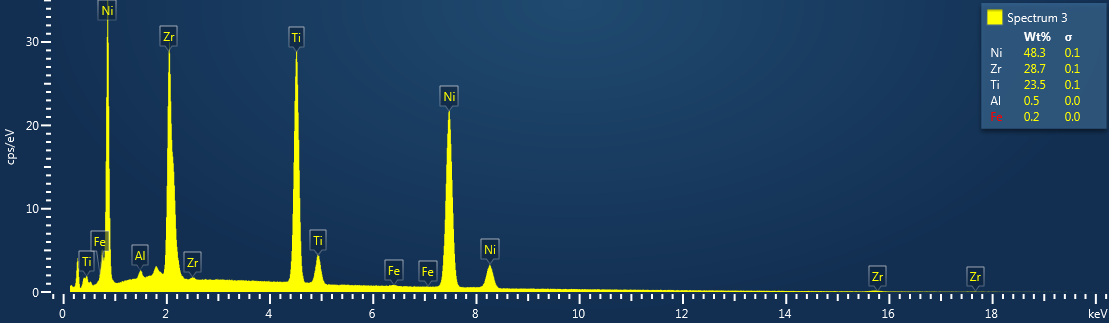
\includegraphics[scale=0.5]{img/dep2.png}
 	\caption{Espectrograma de la cara superior de una muestra de la segunda deposición}
	\label{dep2}
\end{figure} 

En cada muestra se analizaron las caras superiores e inferiores, y cada cara en tres regiones distintas, para estimar diferencias en la variación local de la composición. En las tablas \ref{composition2} y \ref{composition3} pueden verse las diferentes mediciones realizadas.

\begin{table}[H]
\begin{tabular}{c|c|c|c|c|c|c|}
\cline{2-7}
\multicolumn{1}{l|}{} & \multicolumn{3}{c|}{Cara superior} & \multicolumn{3}{c|}{Cara Inferior} \\ \cline{2-7} 
\multicolumn{1}{l|}{} & Region 1 & Region 2 & Region 3 & Region 1 & Region 2 & Region 3 \\ \hline
\multicolumn{1}{|c|}{Ti{[}\%at{]}} & 30,13 & 30,15 & 30,20 & 31,39 & 31,25 & 31,38 \\ \hline
\multicolumn{1}{|c|}{Ni{[}\%at{]}} & 50,56 & 50,56 & 50,53 & 50,23 & 50,27 & 50,22 \\ \hline
\multicolumn{1}{|c|}{Zr{[}\%at{]}} & 19,30 & 19,29 & 19,27 & 18,38 & 18,48 & 18,40 \\ \hline
\end{tabular}
\caption{Medición de composición para una muestra de la segunda deposición en diferentes regiones}
\label{composition2}
\end{table}

\begin{table}[H]
\begin{tabular}{c|c|c|c|c|c|c|}
\cline{2-7}
\multicolumn{1}{l|}{} & \multicolumn{3}{c|}{Cara superior} & \multicolumn{3}{c|}{Cara Inferior} \\ \cline{2-7} 
\multicolumn{1}{l|}{} & Region 1 & Region 2 & Region 3 & Region 1 & Region 2 & Region 3 \\ \hline
\multicolumn{1}{|c|}{Ti{[}\%at{]}} & 33,65 & 33,61 & 33,60 & 32,77 & 32,61 & 32,73 \\ \hline
\multicolumn{1}{|c|}{Ni{[}\%at{]}} & 44,86 & 44,85 & 44,91 & 47,05 & 47,20 & 47,28 \\ \hline
\multicolumn{1}{|c|}{Zr{[}\%at{]}} & 21,49 & 21,54 & 21,50 & 20,17 & 20,19 & 19,99 \\ \hline
\end{tabular}
\caption{Medición de composición para una muestra de la tercera deposición en diferentes regiones}
\label{composition3}
\end{table}

En la Tabla \ref{compositionAvg} se ve el promedio de estas mediciones, y puede apreciarse que la segunda deposición es rica en Ni, mientras que la segunda es pobre en Ni.


\begin{table}[H]
\centering
\begin{tabular}{c|c|c|}
\cline{2-3}
\multicolumn{1}{l|}{} & Deposición 2 & Deposición 3 \\ \hline
\multicolumn{1}{|c|}{Ti{[}\%at{]}} & 30,8 $\pm$ 0,6 & 30,8 $\pm$ 0,4 \\ \hline
\multicolumn{1}{|c|}{Ni{[}\%at{]}} & 50,4 $\pm$ 0,2 & 46 $\pm$ 1 \\ \hline
\multicolumn{1}{|c|}{Zr{[}\%at{]}} & 18,9 $\pm$ 0,5 & 20,8 $\pm$ 0,4 \\ \hline
\end{tabular}
\caption{Composición estimada para ambas deposiciones}
\label{compositionAvg}
\end{table}

Las altas variaciones en la composición entre las diferentes caras de una misma lámina se explican por las variaciones presentes en la potencia de los magnetrones. 

\subsubsection{Difracción de rayos X}
Las láminas depositadas mediante la técnica de magnetrón sputtering no presentan estructura cristalina sin previo tratamiento térmico. En la Figura \ref{amorfo} se muestra el difractograma de una muestra de la tercer deposición sin tratamiento térmico. El resultado es característico de una muestra amorfa. El pico de Si se debe a que este es el material del portamuestras. Resultados similares se hayan en las otras deposiciones.\todo{Qué configuración del equipo?}

\begin{figure}[H]
 	\centering
	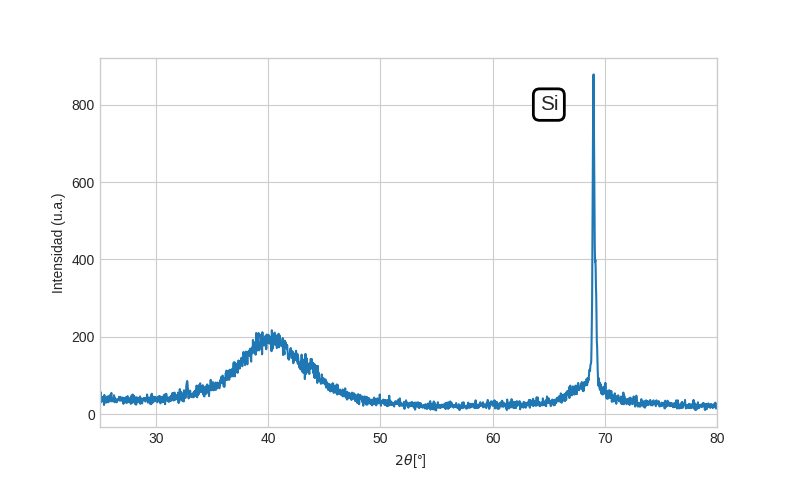
\includegraphics[scale=0.6]{img/RX_amorfo.png}
 	\caption{Difractograma de una muestra de la tercer deposición}
	\label{amorfo}
\end{figure}

\subsection{Temperaturas de cristalización y energía de activación}
\subsubsection{Modelos de Kissinger y Augis-Bennet}
Para determinar la energía de activación de las láminas delgadas de NiTi se trataron térmicamente cinco muestras con DSC a 5, 10, 20, 30 y 50 $^{\circ}/min$. Cada muestra utilizada tenía una masa de 6 mg aproximadamente. El software de adquisición de datos permite realizar un seguimiento de la temperatura y el flujo de calor en función del tiempo, resultando en una tabla del tipo tiempo/temperatura/flujo de calor. El proceso de cristalización, similar para todas fue el siguiente:

\begin{itemize}
\item Se las llevaba a $200^{\circ}C$ a una velocidad de $50^{\circ}C/min$
\item A diversas velocidades por muestra, eran llevadas a $600^{\circ}C$
\item Se bajaba su temperatura a $-50^{\circ}C/min$ hasta $200^{\circ}C$
\item Se las llevaba nuevamente hasta $600^{\circ}C$ a la misma velocidad que fueron llevadas originalmente
\item Finalmente, se llevaba la muestra nuevamente hasta $200^{\circ}C$, momento en el cual finalizaba la medición.
\end{itemize}
En el primer calentamiento hasta $600^{\circ}C$ el objetivo era medir el pico de absorción característico de la muestra. En el segundo calentamiento el objetivo era medir la línea base del equipo. Esto finalmente no se hizo porque\todo{¿por qué quedo como el culo la línea base?}

Debido a que el error relativo de $T_p^{-1}$ es mucho mayor que $ln(\frac{\alpha}{T_p^2})$ y que $ln(\frac{\alpha}{T_p-T_0})$, para poder realizar una regresión lineal se invirtieron los ejes, graficandose así $T_p^{-1}$ en función de $ln(\frac{\alpha}{T_p^2})$ y de $ln(\frac{\alpha}{T_p-T_0})$ para los modelos de Kissinger y Augis-Bennet respectivamente. Esto es
\begin{equation}
	T_p^{-1}=-\frac{R}{E_c}ln(\frac{\alpha}{T_p^2})+cte
\end{equation}

\begin{equation}
	T_p^{-1}=-\frac{R}{E_c}ln(\frac{\alpha}{T_p-T_0})+cte
\end{equation}

Con un ajuste lineal realizado con la función $curve\_fit$ de la librería SciPy se obtuvo el valor de $E_c$ a través de la pendiente en cada modelo. Los puntos calculados a partir de los medidos junto con los ajuste lineales se muestran en las figuras \ref{Kiss} y \ref{AugBen}.


 \begin{figure}[H]
 	\centering
	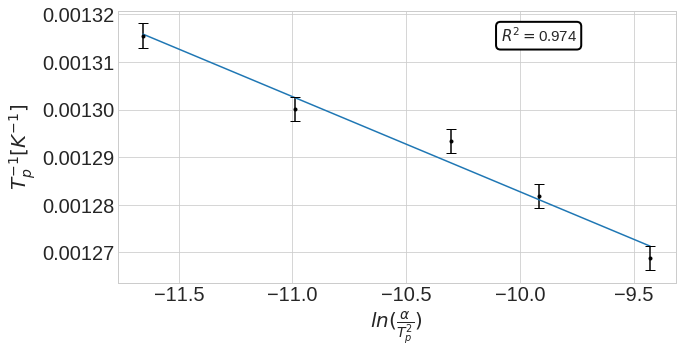
\includegraphics[scale=0.4]{img/Kissinger.png}
 	\caption{Regresión lineal realizada para la relación de Kissinger.}
	\label{Kiss}
\end{figure} 

 \begin{figure}[H]
 	\centering
	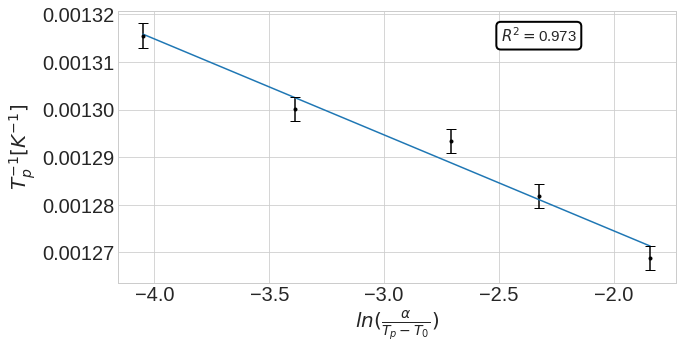
\includegraphics[scale=0.4]{img/Augis_bennet.png}
 	\caption{Regresión lineal realizada para la relación de Augis-Bennet.}
	\label{AugBen}
\end{figure} 


\subsection{Tratamiento térmicos}
Para que las láminas obtenidas presenten una estructura cristalina es necesario realizarles un tratamiento térmico para lograr la cristalización. Las láminas de la segunda y tercera deposición fueron tratadas a $500 ^\circ C$, $600 ^\circ C$, $700 ^\circ C$ y $800 ^\circ C$ dentro de un horno tubular con un controlador de temperatura, sin embargo, para ,mayor precisión en la temperatura, se empleó una termocupla envainada tipo K al lado de la muestra. Cada tratamiento duró una hora.

Cada lámina fue envuelta dentro de una hoja de tantalio y luego encapsuladas, en vidrio para aquellas que iban a $500 ^\circ C$ y $600 ^\circ C$, y em cuarzo para las que iban en $700 ^\circ C$ y $800 ^\circ C$,. Las cápsulas tenían un vació de 3 mTorr en atmósfera de Ar. Esto se realizo para evitar que quedase oxígeno que pudiese oxidar las muestras. Así mismo, el tantalio se eligió porque resiste dichas temperaturas y para que tome el residuo de oxígeno dentro de las capsulas. Aún así, para esta aleación esto parece no haber sido efectivo ya que algunas muestras presentaban una capa de óxido en su superficie, mientras que en la hoja de $Ta$ no se observó ningún tipo de reacción.

Las láminas obtenidas resultaron quebradizas, con lo cual su manipulación resultó ser muy difícil, restringiendo considerablemente los estudios que sobre ellas podían realizarse, especialmente para aquellas de la tercera deposición. Esta fragilidad es atribuible al alto contenido en $Zr$ que presenta la aleación. \todo{Alguién más reporta esto?}

\subsection{Fases obtenidas}
\towrite{Me falta un RX y ni la menor idea de donde sacar los picos.}

\subsection{Temperaturas de transformación}
Para determinar las temperaturas de transformación de las distintas muestras se realizó una calorimetría diferencial de barrido sobre las láminas de la segunda y tercer deposición y sobre las de la segunda deposición, adicionalmente, el método de resistividad por cuatro puntas. En las láminas de la tercera deposición no fue posible realizar este estudio ya que las láminas eran extremadamente frágiles, impidiendo realizar las conexiones necesarias.



\section{Useful tools}
\towrite{an introduction and some examples}

Let's start with the following definition:
\begin{definition}\label{def:domain}
A set $U \in \mathbb{C}$ is a \emph{domain} if:
\begin{itemize}
    \item $U$ is open in $\mathbb{C}$, and
    \item $U$ is connected.
\end{itemize}
\end{definition}


\begin{theorem}[]
Suppose $n \in \mathbb{Z}$, then the following are equivalent:
\begin{enumerate}[label=\roman*.]
    \item $n > 5$.
    \item $5 > 5$.\todo{This doesn't seem right...}
    \item For each $n \in n$, we have:
    \begin{align}\label{eq:truth}
        n > n+1 > n+1^2 > \dots > n+7.
    \end{align}
    where $7$ is an arbitrary element of
    \begin{align*}
        \oint_{a}^{b} \supersine \alpha + i \supercosine \beta  db(a).
    \end{align*}
\end{enumerate}
\end{theorem}

\begin{remark}
Interesting!
\end{remark}
\begin{proof}
%See \cite{Rynne2008LinearAnalysis}.
\end{proof}


\begin{corollary}
Suppose $U \subseteq \mathbb{C}$ is a domain (see Definition \ref{def:domain}), and $f: \overline{U} \rightarrow \mathbb{C}$ is continuous on $\overline{U}$ and holomorphic on $U$. If $z \mapsto |f(z)|$ is constant on $\partial U$, then $f$ has a zero in $U$.
\end{corollary}
\begin{proof}
If not, consider $\frac{1}{f}$.
\end{proof}


\section{Resultados}
\section{Discusión}
\section{Conclusión}
\newpage

% You can choose a citation style, 'plain' is the default
% See:
% https://www.overleaf.com/learn/latex/Bibtex_bibliography_styles
\todo{Make bibliography style consistent. which is the correct one?}
\nocite{*} 
\bibliographystyle{plain}
\bibliography{Referencias}

\end{document}

% Have fun!
% -fons

% http://www2.washjeff.edu/users/rhigginbottom/latex/resources/symbols.pdf